%%%%%%%%%%%%%%%%%%%%%%%%%%%%%%%%%%%%%%%%%%%%%%%%%%%%%%%%%%%%%%%%%%%%%%%%
%%% OpenMDBench --- AAMAS 2027 submission (main paper).
%%% Converted from OpenMDBench0830.md: format changes only (citations
%%% wired to refs.bib, cross-references, booktabs tables, display math).
%%% Domain-specific wording from the draft has been neutralized to
%%% academic terminology (e.g., "rules of interaction",
%%% "coastal/port protection", renamed tactic templates).
%%% Appendices A--H remain in the markdown source as supplementary
%%% material and are cross-referenced via \sapp{...}.
%%%%%%%%%%%%%%%%%%%%%%%%%%%%%%%%%%%%%%%%%%%%%%%%%%%%%%%%%%%%%%%%%%%%%%%%

%%%% For anonymized submission, use this
\documentclass[sigconf,anonymous]{aamas}

%%%% For camera-ready, use this
%\documentclass[sigconf]{aamas}

\usepackage{amssymb}
\usepackage{booktabs}
\usepackage{pifont} % dingbat check/cross marks (LibertinusMath lacks U+2713)
\setlength{\emergencystretch}{3em} % give narrow columns room to break around inline math

%%%%%%%%%%%%%%%%%%%%%%%%%%%%%%%%%%%%%%%%%%%%%%%%%%%%%%%%%%%%%%%%%%%%%%%%

%%% AAMAS-2027 copyright block (do not change!)

\makeatletter
\gdef\@copyrightpermission{
  \begin{minipage}{0.2\columnwidth}
   \href{https://creativecommons.org/licenses/by/4.0/}{
\includegraphics[width=0.90\textwidth]{by}}
  \end{minipage}\hfill
  \begin{minipage}{0.8\columnwidth}
   \href{https://creativecommons.org/licenses/by/4.0/}{This work is licensed under a Creative Commons Attribution International 4.0 License.}
  \end{minipage}
  \vspace{5pt}
}
\makeatother

\setcopyright{ifaamas}
\acmConference[AAMAS 2027]{Proc.\@ of the 26th International Conference
on Autonomous Agents and Multiagent Systems (AAMAS 2027)}{3--7 May 2027}{Hanoi, Vietnam}{M.~Baldoni, F.~Fang, W.~Yeoh, N.~Yorke-Smith (eds.)}
\copyrightyear{2027}
\acmYear{2027}
\acmDOI{}
%\acmPrice{}
\acmISBN{}

%%% Replace with your OpenReview submission id before submitting.
\acmSubmissionID{817}

\submissionType{Research Paper Track}

\title[OpenMDBench]{OpenMDBench: Layering the LLM Only Where It Pays}

%%% Author information is suppressed by the `anonymous' option.
\author{Anonymous Author(s)}
\affiliation{%
  \institution{Anonymous Institution}
  \city{}
  \country{}}
\email{anonymous@example.com}

%%% Notation macros (must precede the abstract, which uses \Cinfo/\Bif).
\newcommand{\sapp}[1]{App.~#1}
\newcommand{\Cinfo}{C_{\mathrm{info}}}
\newcommand{\Bif}{B_{\mathrm{if}}}
\newcommand{\headroom}{\mathrm{headroom}}
\newcommand{\yes}{\ding{51}}
\newcommand{\no}{\ding{55}}

\begin{abstract}
Hybrid stacks that place an LLM deliberator above a small-model executor are the convergent engineering answer for decision problems that separate a slow, semantic deliberation layer from a fast, continuous execution layer; multi-domain adversarial tasks are a primary instance. Yet \emph{when} this layering pays, and \emph{why}, still lacks benchmark-grade evidence. We formalize the two-tier stack as a hierarchical semi-MDP and derive a \emph{conditional layering framework} with three measurable conditions: (i) core difficulty in LLM-strong decision forms, (ii) a goal interface carrying information the executor cannot reconstruct, and (iii) monolithic baseline headroom. \textbf{OpenMDBench}, a distributed open benchmark with central simulation and local inference, validates the framework on two instantiations sharing one interface stack. On a semantically enhanced grid, where decision-form match fails and baseline headroom is insufficient, goal-dose ablations and a live-LLM counterfactual show the interface has a causal contribution yet deployed hybrids trail the strongest pure baseline, the framework's predicted boundary. On a gate-admitted 14-scenario high-fidelity suite, admitted by the pre-registered design-side gates, layered stacks beat the Rule baseline in 11 and the RL baseline in 12 of 14 scenarios, while end-to-end LLM control trails decisively. A mechanism probe shows layered value does \emph{not} require an LLM information advantage: the LLM discriminator underperforms a rule baseline, yet layering still wins; the evidence is more consistent with semantic goal decomposition than with an LLM information advantage. Replay-gated counterfactual attribution localizes failures to planning, execution, or the interface. Our results support a conditional placement principle: in the evaluated cross-domain setting, LLMs are most effective as deliberators above mature executors when decision-form match, interface carrying, and baseline headroom jointly provide room for layered gains.
\end{abstract}

\keywords{multi-agent systems, evaluation benchmark, large language models, hybrid LLM--small model architecture, distributed open evaluation, multi-domain heterogeneous systems}

\begin{document}

\maketitle

\begin{CCSXML}
<ccs2012>
<concept>
<concept_id>10010147.10010178</concept_id>
<concept_desc>Computing methodologies~Artificial intelligence</concept_desc>
<concept_significance>500</concept_significance>
</concept>
<concept>
<concept_id>10010147.10010178.10010224</concept_id>
<concept_desc>Computing methodologies~Multi-agent systems</concept_desc>
<concept_significance>300</concept_significance>
</concept>
<concept>
<concept_id>10010147.10010178.10010224.10010225</concept_id>
<concept_desc>Computing methodologies~Multi-agent reinforcement learning</concept_desc>
<concept_significance>300</concept_significance>
</concept>
</ccs2012>
\end{CCSXML}
\ccsdesc[500]{Computing methodologies~Artificial intelligence}
\ccsdesc[300]{Computing methodologies~Multi-agent systems}
\ccsdesc[300]{Computing methodologies~Multi-agent reinforcement learning}

\section{Introduction}\label{sec:intro}

\paragraph{Two problems, two decision layers.}
Decision problems of interest separate a \emph{deliberation} problem---whom to watch, what to intercept, how to respect interaction protocols, at second-to-minute cycles over semantic, open-ended states---from an \emph{execution} problem---control, tracking, sensing, reactive avoidance, at millisecond-to-second cycles over continuous spaces. In our multi-domain coastal-protection instantiations, the layer boundary coincides with physical-domain boundaries (aerial, surface, shore, underwater). Pure LLM agents cannot meet execution latency and cost budgets; pure RL agents cannot ingest open-ended language objectives or adversarial deception. \textbf{Hybrid stacks---LLMs as deliberators, small models as executors---are the community's convergent response}~\cite{lamarl,lgcmarl,l2m2,reflectivellm}.

\paragraph{Three questions, no ground to answer them.}
If hybridization is the future, benchmark-grade evidence for three questions is conspicuously absent: \textbf{(Q1) Payoff}---does a hybrid outperform the best pure paradigm, and where does it \emph{underperform}? \textbf{(Q2) Necessity}---under what measurable task properties is layering \emph{structurally necessary}? \textbf{(Q3) Bottleneck}---when a hybrid fails, is the fault in planning, execution, or the interface?

The obstacle is infrastructural: the dominant MARL-era benchmarks---from SMAC~\cite{smac} to LLMArena~\cite{llmarena}---inherit the centrally hosted evaluation model. For hybrid systems this fails computationally (hosting billion-parameter LLMs centrally is prohibitive), institutionally (proprietary weights cannot be uploaded), and architecturally (predefined interfaces constrain the composition space hybrid research explores)---so architectures are built with no shared ground to compare them and no instrumentation to tell \emph{why} one wins.

\paragraph{OpenMDBench.}
We resolve the paradox with a requirements-driven pipeline---formalize, build, instrument, validate---whose outputs map one-to-one onto three contributions. Validation runs on two instantiations sharing one interface stack: a semantically enhanced grid maps the law's boundary conditions over ${\sim}1{,}000$ episodes of a complete planner$\times$executor factorial, and a high-fidelity adversarial suite compares five stacks on 14 deception-enabled scenarios under a unified no-intelligence regime. All numbers derive from released per-episode traces.

\paragraph{Contributions.}
Our contributions are threefold, mapping one-to-one onto the pipeline and answering Q1--Q3 in order: the framework predicts \emph{when} layering can pay (Q2), the toolbox localizes \emph{why} a given stack falls short (Q3), and the platform supplies the ground on which both claims are measured (Q1).

\begin{figure*}[!t]
\centering
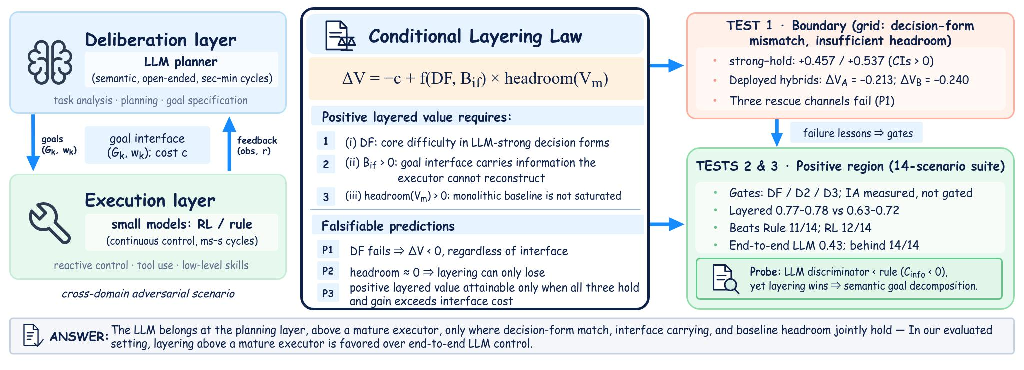
\includegraphics[height=4.5cm]{figures/fig_narrative_overview.pdf}
\Description{Diagram of the conditional layering law: a two-tier decision stack feeds three measurable conditions (decision-form match, interface carrying, baseline headroom), which generate three falsifiable predictions P1--P3. Test 1 (top right) confirms the boundary prediction on the grid (DF fails, headroom insufficient) with specific numbers: strong-hold +0.457/+0.537, deployed hybrids trailing at DeltaVA=-0.213 and DeltaVB=-0.240, three rescue channels failing. Tests 2 and 3 (bottom right) confirm the positive region on the 14-scenario suite: layered 0.77-0.78 vs 0.63-0.72, beating Rule 11/14 and RL 12/14, end-to-end LLM at 0.43 behind 14/14; a mechanism probe shows Cinfo<0 yet layering wins, locating value in semantic goal decomposition.}
\caption{The conditional layering law and its three tests. The two-tier decision stack (left) feeds the law's three measurable conditions (center): decision-form match ($\mathrm{DF}$), interface carrying ($\Bif$), and baseline headroom. \textbf{Test 1} (top right): on the grid boundary regime where decision-form match fails and headroom is insufficient, the goal interface is causally necessary (strong$-$hold: $+0.457/+0.537$, CIs $> 0$) yet deployed hybrids trail the strongest pure baseline ($\Delta V_A = -0.213$; $\Delta V_B = -0.240$); three rescue channels all fail (P1), and the failure lessons harden into pre-registered gates DF/D2/D3. \textbf{Tests 2 and 3} (bottom right): on the gate-admitted 14-scenario high-fidelity suite admitted by the pre-registered design-side gates, layered stacks achieve $0.77$--$0.78$ vs.\ $0.63$--$0.72$ for the monolithic baselines, beating Rule in 11 and RL in 12 of 14 scenarios; end-to-end LLM control trails at $0.43$, behind on 14/14 scenarios. A mechanism probe shows the LLM discriminator underperforms the rule baseline ($\Cinfo < 0$), yet layering still wins---the evidence is more consistent with semantic goal decomposition than with an LLM information advantage.}
\label{fig:law}
\end{figure*}

\textbf{(C1) The conditional layering framework, validated on both sides (Section~\ref{sec:formal}).} From an HSemi-MDP formalization of the two-tier stack and its coupling structure, we derive a \emph{conditional layering law} with three measurable conditions---decision-form match, interface carrying, baseline headroom---and three falsifiable predictions (Figure~\ref{fig:law}). The grid \emph{confirms the boundary prediction}: where decision-form match fails and headroom is insufficient, deployed hybrids trail the strongest pure baseline even though the interface remains causally useful. The gate-admitted high-fidelity suite \emph{provides evidence for the positive-region hypothesis under the pre-registered design-side admission protocol}: admitted by the pre-registered design-side gates, layered stacks beat Rule in 11 and RL in 12 of 14 scenarios. A mechanism probe shows layered value does \emph{not} require an LLM information advantage---locating value in semantic goal decomposition, not perception asymmetry.

\textbf{(C2) A diagnostic toolbox that turns failure analysis into measurement (Sections~\ref{sec:diag}--\ref{sec:exp}).} A replay-gated counterfactual-attribution method decomposing gaps into planning/execution/synergy terms, plus a goal-dose ablation operationalizing $\Bif$ causally. Validated on anchored faults (20/20) and live LLM streams (10/10); they convert where a hybrid fails into per-episode quantities.

\textbf{(C3) OpenMDBench, the experimental substrate (Section~\ref{sec:platform}).} A distributed open platform (simulation central, inference local via polling API) removing the three frictions excluding hybrid systems; it ships two instantiations sharing one interface stack, a 36-scenario family, layered metrics, and trace release. The platform is the precondition on which C1--C2 are measurable, and together they answer where the LLM should sit.

\paragraph{Paper organization.}
Section~\ref{sec:related} positions related work; Section~\ref{sec:formal} formalizes problem and coupling theory; Sections~\ref{sec:platform}--\ref{sec:diag} present platform and diagnostics; Section~\ref{sec:exp} validates; Sections~\ref{sec:discussion}--\ref{sec:conclusion} discuss and conclude. Results derive from released per-episode traces and manifests.

\section{Related Work}\label{sec:related}

\paragraph{MARL benchmarks.}
Classic cooperative MARL benchmarks~\cite{smac,smacv2} and continuous-control environments such as Google Research Football~\cite{grf} standardize comparison in single domains with homogeneous agents; heterogeneity~\cite{hemac,lshc,poac}, application~\cite{ape,hivex}, social-dilemma~\cite{meltingpot}, and standardization~\cite{pettingzoo,benchmarl,marllib} remain single-domain and platform-hosted; BenchMARL~\cite{benchmarl} further advances standardized and reproducible benchmarking across MARL algorithms and environments. Existing work has demonstrated LLM--MARL hierarchical architectures~\cite{lamarl,lgcmarl,l2m2,reflectivellm}, but existing benchmark suites do not systematically evaluate \emph{when} such layering is beneficial, \emph{when} it fails, or \emph{which} layer is responsible for the failure.

\paragraph{LLM agent benchmarks.}
General LLM-agent benchmarks---AgentBench~\cite{agentbench}, WebArena~\cite{webarena}, GAIA~\cite{gaia}---measure task completion across web, tool-use, and knowledge domains. Interactive-LLM multi-agent benchmarks~\cite{llmarena,multiagentbench,mindagent,decrypto,spinbench} evaluate LLM agents but run the LLM on the platform side---the inverse of our distributed paradigm---and none spans multiple physical domains or evaluates hybrid stacks; surveys map this fragmented landscape~\cite{llmagentsurvey25}. Position work argues executable agent evaluation suffers an \emph{identification problem}: benchmark scores and leaderboard rankings can be sensitive to seemingly minor evaluation conventions~\cite{whenbenchtargets}, motivating tighter control of non-model evaluation components~\cite{whenbenchtargets}---the agenda OpenMDBench implements (C3).

\paragraph{Hybrid LLM--small model architectures.}
Compositional designs---CICERO~\cite{cicero22}, LLM controllers over specialized models~\cite{hugginggpt23}, reasoning-action interleaving~\cite{react}, cognitive-architecture frameworks~\cite{coala}, hierarchical HTN-LLM planners~\cite{chathtn25}, and LLM-RL combinations~\cite{lamarl,lgcmarl,l2m2,reflectivellm}---converge on the same placement: the LLM deliberates above a mature executor, in line with the LLM-Modulo position that LLMs cannot autonomously plan but can \emph{help} planning~\cite{kambhampati24} and critical audits of end-to-end LLM planning~\cite{valmeekam23}. The hierarchical structure traces to the Options/Semi-MDP framework~\cite{sutton99}; we add a semantic goal interface and derive empirical conditions for when the upper layer pays. What this line lacks is benchmark-grade evidence for \emph{when} the placement pays---the gap our conditional layering law fills (C1).

\paragraph{Adversarial and security evaluation.}
Network-security RL environments such as CyberBattleSim~\cite{cyberbattlesim} study deception in single-domain settings with RL agents; LLM cyber agents~\cite{rigaki23} deploy LLMs directly as attackers in NetSecGame, and DefenderBench~\cite{defenderbench} evaluates LLM language agents across offense, defense, and knowledge tasks---yet all remain single-domain, treat LLM agency as beneficial by default, and none measures when a layered stack outperforms a monolith. Our asymmetric coastal-protection suite extends adversarial evaluation across physical domains (aerial, surface, shore, underwater) with a standardized scripted opponent and deception-by-construction templates, explicitly testing the conditional value of layering rather than assuming it.

\paragraph{Multi-agent attribution and failure diagnosis.}
Counterfactual credit assignment originates in MARL with COMA~\cite{coma}. Subsequent tools decompose outcomes across agents~\cite{triantafyllou25}, quantify emergent synergy~\cite{weinberg25}, localize Patient-0 failures~\cite{shefin26}, and score module contributions inside an LLM agent~\cite{capa25}---all explain \emph{agents}, \emph{policies}, or \emph{modules}; none is replay-gated, validates on real LLM streams, or ships as a standard protocol. To our knowledge, our $\Delta P/\Delta E/\Delta I$ counterfactual contribution decomposition is the first \emph{replay-gated} protocol localizing planning-vs-execution contributions on \emph{live} LLM streams (10/10) and anchored faults (20/20) as a built-in benchmark component (C2).

\paragraph{Distributed and federated evaluation.}
Distributed computation in RL has been training-side~\cite{gorila,impala,a3c,fedrlsurvey}; OpenFedLLM~\cite{openfedllm} federates LLM \emph{training}. To our knowledge, no prior benchmark runs simulation centrally while agent inference runs locally---a new evaluation paradigm for hybrid systems.

\paragraph{Comparison.}
Table~\ref{tab:comparison}: to our knowledge, no existing benchmark combines multi-domain heterogeneity, hybrid-architecture support, natural-language task interfaces, and open evaluation.

\begin{table}[t]
\centering
\caption{OpenMDBench vs.\ representative benchmarks.}
\label{tab:comparison}
\resizebox{\columnwidth}{!}{%
\footnotesize
\setlength{\tabcolsep}{3pt}
\begin{tabular}{@{}llllccc@{}}
\toprule
Benchmark & Domain & Agent type & Execution & LLM & Hybrid & NL \\
\midrule
SMAC~\cite{smac} & Single & Homog.\ MARL & Local environment & \no & \no & \no \\
LLMArena~\cite{llmarena} & Single & Pure LLM & Benchmark-side & \yes & \no & \yes \\
MultiAgentBench~\cite{multiagentbench} & Diverse & Pure LLM & Benchmark-side & \yes & \no & \yes \\
SPIN-Bench~\cite{spinbench} & Multi-domain & Pure LLM & Benchmark-side & \yes & \no & \yes \\
\midrule
\textbf{OpenMDBench} & \textbf{Multi-domain} & \textbf{Hybrid} & \textbf{Central sim / local inference} & \textbf{\yes} & \textbf{\yes} & \textbf{\yes} \\
\bottomrule
\end{tabular}}
\end{table}

\section{Problem Definition: Decision-Stack Bifurcation and Formalization}\label{sec:formal}

\subsection{The Two Layers}\label{sec:layers}

The problem bifurcates by cycle and state type: a \emph{deliberation layer} over semantic state at second-to-minute cycles (mission understanding, cross-domain allocation, intent inference, protocol compliance, replanning) and an \emph{execution layer} over continuous state at millisecond-to-second cycles (control, tracking, sensing, reactive tactics)---a property of the problem, not the solver.

\subsection{HSemi-MDP Formalization}\label{sec:hsemimdp}

We formalize as a \textbf{hierarchical semi-MDP} $M = \langle M_d, \{M_e^k\}, G \rangle$: an upper deliberation Semi-MDP $M_d$ over semantic state (allocation, task progress, opponent belief, rules) with event-driven goal-assignment actions at random inter-decision intervals; a lower execution-MDP family $M_e^k$ per domain with continuous dynamics and rewards parameterized by goals $(G_k, w_k)$ handed down from above. The interface carries explicit cost $c \geq 0$---goal-conditioned execution is weaker than an unconstrained monolith when goals carry no exploitable information, reconciling why layering can hurt. A scripted opponent standardizes scenarios; its strength knobs calibrate headroom.

\subsection{Cross-Domain Coupling and the Layering Law}\label{sec:law}

A key structural parameter is \textbf{cross-domain coupling}---how much upper-layer decisions coordinate across domains. We measure it as effective coupling, the mean number of domains touched per allocation decision, observable from execution traces; intrinsic task coupling (minimum required domain count $\times$ inter-domain dependency strength) bounds it from above. Coupling enters the law indirectly: it raises the ceiling on what the interface can carry (a goal stream coordinating more domains lifts the upper bound on $\Bif$) and shapes which decision forms dominate planning, modulating $\mathrm{DF}$.
\paragraph{Operationalizing the coupling terms.}
Two quantities anchor the law. \textbf{Interface information} $\Bif$, the effective information carried by the goal interface, is operationalized \emph{causally} as the paired performance cost of disabling the interface (the goal-dose ablation of Section~\ref{sec:goaldose}), not by an observational estimate. \textbf{Channel information asymmetry} $\Cinfo$, the information asymmetry between the two observation channels, is probed \emph{behaviorally} through discrimination performance on the public channel. $\Cinfo$ is \emph{not} a condition of the law but a competing mechanism hypothesis (whether layered value requires an LLM information advantage), tested in Section~\ref{sec:mechanism} and reframed there as a reported diagnostic rather than a gate. Both are grid-side instruments; the high-fidelity suite relies on the pre-registered gates (Section~\ref{sec:hifi}).

\paragraph{The layering law.}
Let $V_m$ be the best \emph{pure-execution} (monolithic) baseline and $\Delta V = V_{\mathrm{hybrid}} - V_m$. Under the time-scale separation of Section~\ref{sec:layers}, the hybrid value decomposes into an executor floor $V_m$, an interface constraint cost $-c \leq 0$ (goal-conditioned execution cannot exceed an unconstrained monolith unless goals carry exploitable information), and a planner's gross gain. Two forces bound that gain: the executor absorbs at most a fraction $f(\mathrm{DF},\Bif)$ of it---zero when the core difficulty is not in LLM-strong decision forms ($\mathrm{DF}$) or the interface carries nothing the executor cannot reconstruct ($\Bif$)---and the gain cannot exceed the headroom $\headroom(V_m)$ the baseline leaves below the oracle $V^*$. Assembling the two bounds yields the conditional form
\begin{equation}
\!\Delta V = -c\!+\!f(\mathrm{DF},\Bif)\,\headroom(V_m)\!
\label{eq:law}
\end{equation}
with $\headroom(V_m) = (V^* - V_m)/(V^* - V_{\min})$, the normalized gap to oracle---the worst-baseline denominator removes absolute-scale dependence, so headroom is comparable across scenarios of different difficulty---and $f \geq 0$ increasing in both arguments. Here $\mathrm{DF}$ denotes \emph{decision-form match}: the task's core difficulty must reside in semantic decision forms the LLM handles well (allocation, intent inference, protocol compliance), not in spatial micro-control where small models are stronger.

\paragraph{Why each condition is necessary.}
The three conditions are not independent heuristics; each is motivated by the HSemi-MDP structure and the semantic-goal interface design. \textbf{(i) Decision-form match.} If the core bottleneck lives in the execution layer (geometric micro-control), the goals handed down by the upper layer are information the executor cannot exploit---it is already saturating on kinematics, not waiting for guidance---so $\Bif \to 0$ and $f \to 0$, leaving $\Delta V = -c$: layering adds only interface cost. \textbf{(ii) Interface carrying.} If the goal interface does not carry information the executor could not reconstruct itself---the LLM merely restates state the executor already observes---then the upper layer contributes nothing beyond the monolithic baseline, and again $\Delta V = -c$. A third route to the same outcome is an \emph{executor floor}: when the executor saturates at a performance floor, goals cannot rescue it and $\Bif \to 0$ regardless of what the interface carries (Section~\ref{sec:boundary}). \textbf{(iii) Baseline headroom.} If the monolithic baseline is already near oracle ($\headroom \approx 0$), even a positive $f(\mathrm{DF},\Bif)$ is multiplied by $\headroom \approx 0$, and again $\Delta V \approx -c$. The law's falsifiable content is therefore that $\Delta V > 0$ requires all three to hold jointly (necessary, not sufficient: the planner gain must also exceed the interface cost $c$); violating any one reduces the second term to zero and layering can only lose.

Eq.~\ref{eq:law} fixes the \emph{directional} structure; we deliberately do not fit $f$ or estimate $c$ in absolute terms (Section~\ref{sec:limitations}). Prior unconditional formulations (``advantage scales positively with coupling'') omit decision-form match and headroom and are refuted by our boundary-regime experiments: the interface is causally necessary (Section~\ref{sec:goaldose}), yet at a near-saturated baseline with a decision-form mismatch both deployed hybrids sit significantly \emph{below} it---layering only loses where the conditions fail and pays where they jointly hold (Sections~\ref{sec:boundary}--\ref{sec:hifiresults}). Figure~\ref{fig:law} summarizes the law and the three falsifiable predictions below.

\paragraph{Performance accounting.}
A $2\times2$ deployment accounting identity (planner/executor swap contrasts $P,E,I$ vs.\ the strongest pure baseline) fixes the threshold layering must clear (Table~\ref{tab:sixarm}; full derivation: \sapp{I}).

\paragraph{Design corollaries (pre-registered acceptance gates).}
The law converts into falsifiable environment requirements enforced before any full-scale run: \textbf{(DF)} decision-form match (operationalized as a myopic greedy allocation script scoring $<$ 90\% of the rule baseline), \textbf{(D2)} headroom (best pure baseline SR $\in [40\%, 85\%]$), and \textbf{(D3)} interface budget (goal-dose effects exceeding seed-level variance). Information asymmetry (IA) is measured but not gated (Section~\ref{sec:mechanism}); Section~\ref{sec:interface} shows the DF-violation case, and Section~\ref{sec:hifi} embeds DF/D2/D3 into the high-fidelity protocol.

\paragraph{Three falsifiable predictions.}
The law converts into three testable predictions: \textbf{(P1)} at a decision-form mismatch ($\mathrm{DF}$ fails), the planner-side gain vanishes, so $\Delta V \le -c$; \textbf{(P2)} at a saturated baseline ($\headroom \approx 0$), layering can only lose; \textbf{(P3)} positive layered value is attainable only in the joint-positive region of all three conditions; outside that region, positive value is structurally ruled out under the model assumptions. Section~\ref{sec:exp} tests each: P1--P2 on the grid's boundary regime, P3 on the gate-admitted high-fidelity suite.



\section{The OpenMDBench Platform}\label{sec:platform}

\subsection{Distributed Open Evaluation Architecture}\label{sec:arch}

The \textbf{Central Simulation Server (CSS)} maintains environments, generates briefings, executes actions, and computes metrics. \textbf{User-Local Hybrid Agents (ULHAs)} run all inference locally behind a standardized \textbf{polling API} (RESTful HTTP, JSON; \sapp{B}); simulation advances asynchronously of inference and sessions are resumable. This removes the three frictions excluding hybrid systems from prior benchmarks: no weights cross the trust boundary, users bear inference cost, and the composition space stays open. Integrity is enforced by protocol rather than trust: rate limits and action-pattern checks bound the trust model, manifest-hash freezing fixes versions, and determinism gates plus channel-fairness audits equalize what each stack sees (\sapp{B}, \sapp{H}).

\begin{figure*}[t]
\centering
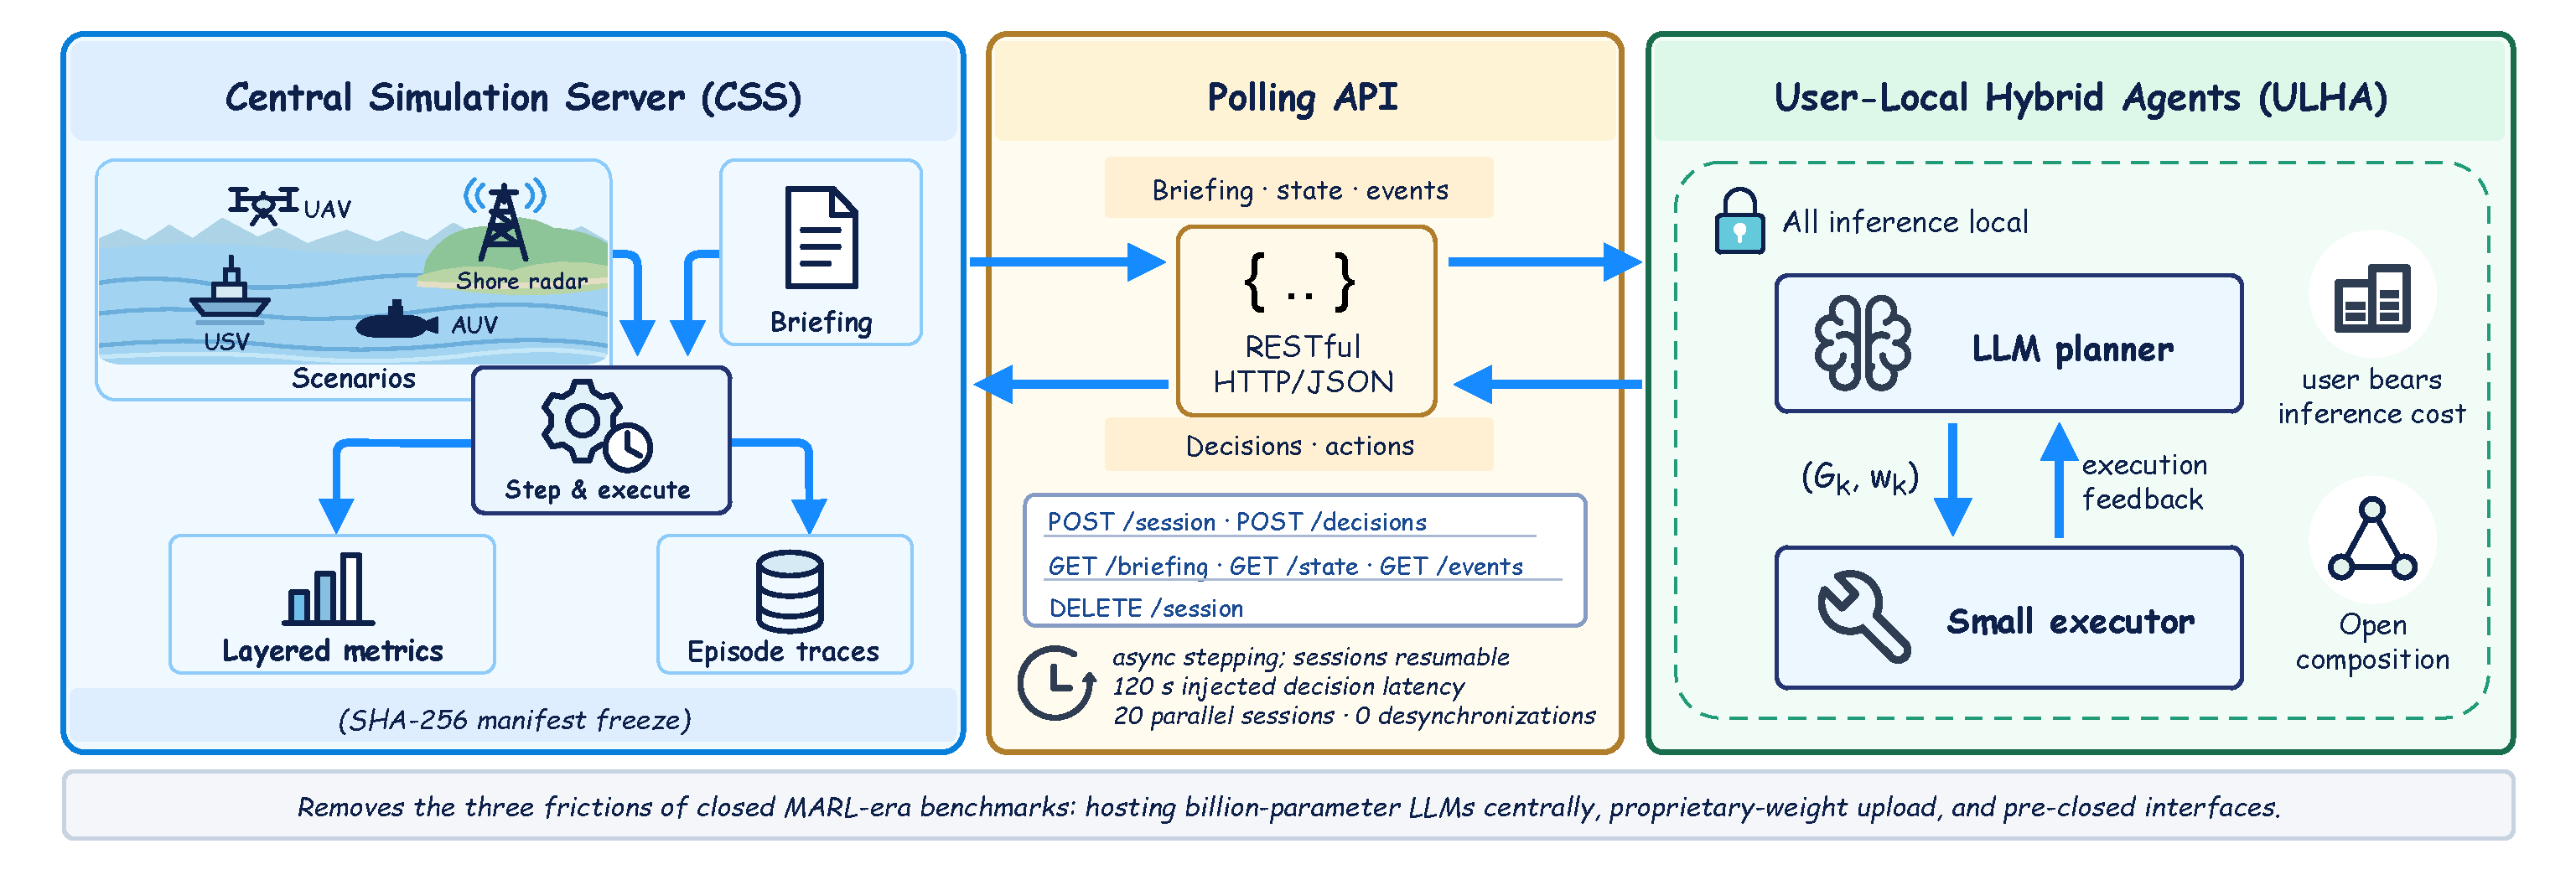
\includegraphics[height=4.2cm]{figures/fig_arch.pdf}
\Description{Schematic of the distributed open evaluation architecture: a central simulation server maintains environments, briefings, and metrics while user-local hybrid agents run all inference behind a polling API; no weights cross the trust boundary and sessions are resumable.}
\caption{Distributed open evaluation architecture: simulation and metrics central (CSS); all inference local behind a polling API (ULHA).}
\label{fig:arch}
\end{figure*}

\subsection{Scenario Family and Task Suite}\label{sec:scenario}

We instantiate an \textbf{asymmetric coastal-protection} family: Red (defender, evaluated) fields UAVs, USVs, shore radar, and AUVs (heterogeneous, complementary sensing); Blue (scripted opponent) uses tactic templates with calibrated strength knobs (\sapp{C}). 36 scenarios across 5 categories (reconnaissance, tracking \& surveillance, interception \& response, zone control, emergency response) at 3 difficulties, each requiring cross-domain coordination. Two instantiations share the interface stack: a \textbf{high-fidelity continuous-dynamics suite} (14 gate-admitted scenarios, deception by construction; Section~\ref{sec:hifi}) and a \textbf{semantically enhanced grid-world} (50\% feints indistinguishable by numeric features, intercepting a feint is an own-goal; \sapp{H}).

\subsection{Layered Evaluation Metrics}\label{sec:metrics}

From $\sim$40 raw per-episode measures we compute planning-attributable, execution-attributable, and composite scores (0.5/0.5 default), aggregated with paired statistics (Wilcoxon, sign tests, bootstrap CIs; full definitions: \sapp{E}). All stacks run under a \emph{unified no-intelligence regime}---identical briefings, prompts, and channels---so contrasts isolate architecture, not prompt engineering. These scores decompose where performance is earned statically; counterfactual attribution (Section~\ref{sec:attribution}) is a separate instrument replacing the upper layer to measure causal contribution.

\section{Diagnostic Instrumentation}\label{sec:diag}

Ranking cannot answer Q3. Unlike the $2\times2$ deployment accounting identity (Section~\ref{sec:law}), which accounts components statically, counterfactual attribution \emph{replaces} components to measure causal contribution. Two causal tools exploit the HSemi-MDP structure and directly validate the law's conditions: the goal-dose ablation operationalizes $\Bif$ causally (condition ii), and the $\Delta P/\Delta E/\Delta I$ decomposition---if gains concentrate in $\Delta P$, the LLM's contribution is in planning (condition i's mechanism), not execution or interface artifact.

\subsection{Counterfactual-Replay Attribution}\label{sec:attribution}

\paragraph{Method.}
For a system $(\pi_d, \pi_e)$ with performance $V(\pi_d, \pi_e)$, we construct three counterfactuals: (1) \emph{reference-execution replay}---enforce the recorded upper decisions $D = \{(t_m, a_d^m)\}$ at the same times while replacing execution with an independently validated reference executor $\pi_e^*$; (2) \emph{reference planning}---replace $\pi_d$ with a reference planner $\pi_d^*$ keeping $\pi_e$; (3) \emph{reference full stack}. In the grid experiments $\pi_d^*$ is the rule planner, $\pi_e^*$ the GOAI heuristic executor, and the reference full stack the Rule baseline (\sapp{I}). The asymmetry follows from time-scale separation: upper decisions are sparse, so fixing their sequence does not over-constrain; lower actions are dense, so fixing them would erase the policy. The decomposition reads:
\begin{align}
\Delta E &= V(\pi_d,\pi_e) - V(\pi_d,\pi_e^*) \quad \text{(execution)},\label{eq:de}\\
\Delta P &= V(\pi_d,\pi_e) - V(\pi_d^*,\pi_e) \quad \text{(planning)},\label{eq:dp}\\
\Delta I &= V(\pi_d^*,\pi_e^*) - V(\pi_d^*,\pi_e) - V(\pi_d,\pi_e^*) \nonumber\\
&\quad + V(\pi_d,\pi_e) \ \text{(synergy)}.\label{eq:di}
\end{align}
The method is \emph{replay-gated}: a contrast is admitted only after the original episode and every counterfactual pass exact-replay verification---the replayed sequence reproduces the recorded trajectory---so no contrast rests on behavior the system never produced. Positive $\Delta P$ ($\Delta E$) means the deployed planner (executor) beats the reference on the same partner; $\Delta I$ is the interaction term, maximal when both layers are individually inert but jointly improving.

\paragraph{Validity and preconditions.}
Five pre-registered checks guard the decomposition (\sapp{D}); injected-bottleneck validation localizes 20/20 anchored faults under those gates (Section~\ref{sec:attrval}). It requires a goal-responsive executor and deterministic dynamics (satisfied by the grid); the real-stream counterfactual validates on live LLM planning streams, while the nondeterministic endpoint uses the prompt-level audit.

\subsection{Goal-Dose Interface Ablation}\label{sec:goaldose}

$\Bif$ is operationalized causally via paired strong-vs-hold interface conditions (mask1/mask2 dose tiers replace goals with legal holds); the strong--hold contrast estimates the goal stream's total contribution. Replaced commands are legal actions, so the intervention changes what the interface carries, not whether the executor can act. Doses are unit-availability, not bits (\sapp{D}).

\section{Validation: Boundary Regime and Positive Region}\label{sec:exp}

We now validate the entire pipeline and pin down the layering law's boundary regime. \emph{All numbers derive from released per-episode traces; every table is paired by seed.}

\subsection{Setup}\label{sec:setup}

Systems: pure RL (MAPPO, goal-conditioned), rule (scripted planner), pure LLM (low-level actions), hybrid (LLM planner over MAPPO or heuristic executors; Qwen3.8-27B, temp 0.1 for grid experiments; high-fidelity evaluation uses temp 0.0). All contrasts are within-batch, paired on shared seeds, with seed-bootstrap 95\% CIs (\sapp{F}): ten paired seeds per medium-tier batch (goal-dose, six-arm, real-stream), five per complex batch (Section~\ref{sec:payoff}).

\subsection{Grid: Boundary Confirmation}\label{sec:payoff}

\paragraph{Difficulty cliff.}
Across tiers, pure MAPPO scores 100\% / $\approx$97\% / \textbf{0\%} vs.\ rule 100\% / 97\% / \textbf{65\%}: the complex tier's deception load (indistinguishable feints, anomaly relabeling, interference) collapses end-to-end small models yet survives orchestration---exactly the difficulty a deliberator is meant to carry.

\paragraph{The $2\times2$ factorial isolates the executor floor.}
On complex, every MAPPO-executor stack scores 0\%; with the heuristic executor, rule reaches 65\% and LLM 5\%. The MAPPO executor is the observed bottleneck under the frozen training protocol; a diagnostic re-training audit (12 configurations) confirms the 0\% is robust across current hyperparameters---frozen-medium transfer collapses after on-complex fine-tuning, evidence of training dynamics, not task unsolvability (\sapp{F}).

\paragraph{Complex-layer layered stacks confirm the P1 prediction directly.}
A frozen five-seed paired batch (63101--63105) ran all four stacks on complex with one fixed medium checkpoint (\sapp{F}): LLM+heuristic scores 0.400 vs.\ Rule 0.787 (paired $\Delta V = -0.387$, CI $[-0.707, -0.053]$), and LLM+MAPPO 0.220 vs.\ Pure MAPPO 0.240 ($\Delta V = -0.020$, CI $[-0.073, +0.027]$). Two mechanisms surface: where the decision form is a mismatch (geometric micro-control), the LLM planner \emph{hurts}---the same heuristic executor drops from 0.787 (rule goals) to 0.400 (LLM goals); where the executor is the bottleneck (MAPPO at 0\%), adding the LLM changes nothing. The medium-tier six-arm accounting shows the same direction ($\Delta V_A = -0.213$), the monotonic worsening being exactly the P1 gradient (\sapp{F}).

\paragraph{Tournament.}
Round-robin Elo: pure RL $\approx$ hybrid (1555 vs.\ 1553) $>$ rule $\gg$ pure LLM $>$ random---the grid's boundary outcome, violating DF (geometric interception) and D2 (saturated baseline; \sapp{F}).

\subsection{Attribution Validation}\label{sec:attrval}

On injected-bottleneck calibration the method passes all five pre-registered gates (\sapp{D}) and localizes 20/20 anchored faults (full table: \sapp{I}). A 12-episode natural-failure pilot agrees with human annotation in 4/12 ($\kappa=0.25$); disagreements are semantic---the $\Delta I$ marginal-interaction label is read by humans as ``balanced''---confirming $\Delta I$ measures layer interaction, not first-order fault location.

\subsection{Grid Boundary: Interface Necessary but Insufficient}\label{sec:boundary}

Three paired batches on medium tier (10 seeds each): goal-dose, six-arm (Table~\ref{tab:sixarm}), real-stream counterfactual.

\textbf{The goal interface has a causal contribution under the paired intervention.} Disabling it collapses performance: strong$-$hold $= +0.457$ (rule) / $+0.537$ (LLM), both CIs above 0; under hold both score 0.213 and become indistinguishable; the real-stream counterfactual agrees (10/10 seeds, $+0.420$).

\textbf{Headroom boundary (P2): interface necessity does not clear a saturated baseline.}
Against the strongest pure baseline ($V_m=0.913$), both deployed hybrids sit significantly below it (Table~\ref{tab:sixarm})---a near-saturated baseline leaves little headroom. The same prediction holds inside the positive region: IE-03, the only admitted scenario with a near-saturated RL baseline (0.96), is where layering does not pay; across the family layered gain trends negatively with headroom (Spearman $\rho=-0.50$ LLM+Rule, $-0.68$ LLM+RL; \sapp{A}).

\textbf{The dose--gain curve anchors the law's increasing branch.}
Across four paired doses (hold, mask2, mask1, strong), both stacks improve significantly from hold to mask1 but not monotonically beyond---``more interface is always better'' is refuted (full table: \sapp{I}).

\begin{table}[t]
\centering
\caption{Six-arm accounting batch (medium tier, 10 paired seeds): mean composites and per-seed successes, with deployment accounting identities (seed-bootstrap 95\% CIs). $V_m$ = per-seed max of pure baselines (rule+rule overall mean 0.913; pure RL overall mean 0.883).}
\label{tab:sixarm}
\resizebox{\columnwidth}{!}{%
\footnotesize
\begin{tabular}{@{}lcccl@{}}
\toprule
Stack & Mean $V$ & Succ. & Identity & [95\% CI] \\
\midrule
rule+rule ($V_{\mathrm{RR}} = V_m$) & 0.913 & 9/10 & --- & --- \\
pure RL & 0.883 & 9/10 & --- & --- \\
rule+RL ($V_{\mathrm{RM}}$) & 0.810 & 8/10 & $E = -0.103$ & $[-0.263, +0.000]$ \\
LLM+rule ($V_{\mathrm{LR}}$) & 0.700 & 6/10 & $P = -0.213$ & $[-0.497, +0.080]$ \\
LLM+RL ($V_{\mathrm{LM}}$) & 0.673 & 6/10 & $I = +0.077$ & $[-0.240, +0.380]$ \\
pure LLM & 0.280 & 1/10 & --- & --- \\
\midrule
\multicolumn{5}{@{}l}{$B = V_m - V_{\mathrm{RR}} = 0$;\ $\Delta V_A = P - B = -0.213$ $[-0.497, -0.037]$;}\\
\multicolumn{5}{@{}l}{\hspace*{2em}$\Delta V_B = P + E + I - B = -0.240$ $[-0.490, -0.087]$}\\
\bottomrule
\end{tabular}}
\end{table}

\textbf{The law's interface conditions reproduce across models.}
A four-model scan (two dense, two MoE) reproduces interface necessity in 4/4 and the deployment deficit in 3/4; the fastest MoE reaches the pure-RL level in strong condition---a headroom boundary, not a violation (\sapp{F}).

\subsection{Decision-Form Anatomy (P1)}\label{sec:intervention}

Three pre-registered rescue channels---information injection, replanning frequency, interface modality---all fail on the complex tier: the LLM reads and cites the intelligence yet performance does not move, tracing the deficit to semantic-to-geometric conversion under spatial-combinatorial load. The pattern is robust across training configurations (Section~\ref{sec:payoff}), motivating $\mathrm{DF}$ as the law's first condition. The two negative conditions separate cleanly: interface strength cannot rescue a decision-form mismatch (P1), while a strong interface at a saturated baseline still cannot pay (the fastest MoE reaches only the pure-RL level under strong; Section~\ref{sec:boundary}, P2)---each prediction bites independently (details: \sapp{H}).

\subsection{Interface Modality}\label{sec:interface}

Interface choice is load-matched (\sapp{H}): JSON wins at low semantic load, NL recovers at high load, neither rescues an overmatched planner. A replanning-frequency sweep plateaus at 5-step cycles while cost grows 2.5$\times$; no frequency reaches the pure-RL baseline---bandwidth cannot substitute for missing headroom (P2).

\subsection{From Boundary Conditions to the Gates}\label{sec:hifi}

The grid results convert into pre-registered acceptance gates (DF/D2/D3; Section~\ref{sec:law}): decision-form match, headroom, and interface budget, with IA measured but not gated. The main run was preceded by determinism gates, channel-fairness audits, and manifest-hash freezing.

\paragraph{Scope and honesty of the gated design.}
The gates are a \emph{pre-registered design choice}, not post-hoc filtering: they were frozen before the high-fidelity run, so the 14 admitted scenarios are not cherry-picked for layered performance. We acknowledge the circularity: the positive region is confirmed on scenarios selected to satisfy the law's conditions---the intended test of P3, not an unbiased survey of the family. A 7-scenario sensitivity check bounds the design effect: layered gain is uncorrelated with the DF prior ($\rho=-0.009$, range $[-0.030,+0.086]$), so the law's predictions do not reduce to the gate threshold itself (\sapp{A}). D2/D3-excluded scenarios were not run with layered stacks (that family ships only script policies, and existing weights would conflate ``executor does not know this task'' with ``no headroom''); the negative side of P3 is thus supported by the grid boundary regime and IE-03 (future work: executor re-training). A headroom probe confirms the family cannot resolve this dimension: in IE-05, degrading planning information collapses every tier to a structural floor ($V \approx 0.18$); P3's negative side is untestable within-family (\sapp{F}).

\subsection{Tests 2 and 3: the Positive Region and its Refinement}\label{sec:hifiresults}

14 scenarios, five stacks (two layered, end-to-end LLM, two monolithic baselines), unified no-intelligence regime, five seeds per LLM stack, three-part stability criterion (Table~\ref{tab:hifi}; Figure~\ref{fig:hifigap}: end-to-end gap).

\begin{table*}[t]
\centering
\caption{High-fidelity suite (14 scenarios, unified no-intelligence regime): composite defender score; \textbf{bold} = best. Five seeds per LLM stack (7/11/13/17/19), one replication under nondeterminism; rule/RL never read the briefing (frozen archive, SHA-256 verified); LLM+RL uses one locked checkpoint. \emph{Overall}: mean $\pm$ sd over 14 scenario means.}
\label{tab:hifi}
\footnotesize
\setlength{\tabcolsep}{3pt}
\begin{tabular}{@{}lccccc@{}}
\toprule
Scenario & LLM+Rule & LLM+RL & Pure LLM & Rule & RL \\
\midrule
IE-01 single target & \textbf{0.900} & 0.774 & 0.343 & 0.691 & 0.876 \\
IE-02 dual threat & \textbf{0.908} & 0.851 & 0.162 & 0.765 & 0.757 \\
IE-03 surface raid & 0.856 & 0.634 & 0.699 & 0.748 & \textbf{0.960} \\
IE-04 combined arms & 0.710 & 0.804 & 0.246 & \textbf{0.812} & 0.687 \\
IE-05 multi-axis & 0.790 & \textbf{0.824} & 0.188 & 0.763 & 0.703 \\
IE-06 decoy mixed & 0.767 & \textbf{0.793} & 0.434 & 0.657 & 0.652 \\
IE-07 cross-domain & \textbf{0.792} & 0.763 & 0.703 & 0.749 & 0.684 \\
IE-08 island strike & 0.404 & \textbf{0.568} & 0.280 & 0.432 & 0.301 \\
IE-09 staggered waves & \textbf{0.880} & 0.859 & 0.638 & 0.820 & 0.629 \\
IE-10 dual-axis pincer & 0.712 & \textbf{0.921} & 0.603 & 0.801 & 0.729 \\
IE-11 decoy screen & 0.747 & \textbf{0.820} & 0.346 & 0.681 & 0.184 \\
IE-12 fog onset & \textbf{0.766} & 0.659 & 0.441 & 0.711 & 0.641 \\
IE-13 deep strike & \textbf{0.807} & 0.790 & 0.597 & 0.709 & 0.538 \\
IE-14 saturation & 0.793 & \textbf{0.897} & 0.354 & 0.787 & 0.506 \\
\midrule
\emph{Overall} & 0.774 $\pm$ 0.124 & \textbf{0.783 $\pm$ 0.100} & 0.431 $\pm$ 0.187 & 0.723 $\pm$ 0.098 & 0.632 $\pm$ 0.203 \\
\emph{Mean wins vs.\ Rule} & 11 & 11 & 0 & -- & -- \\
\emph{Mean wins vs.\ RL} & 12 & 12 & 4 & -- & -- \\
\bottomrule
\end{tabular}
\end{table*}


\textbf{Layering wins where the gates hold.} Each layered stack beats the Rule baseline in 11 of 14 scenarios and the RL baseline in 12 of 14 (overall 0.77--0.78 vs.\ 0.63--0.72; Table~\ref{tab:hifi}); the stricter every-seed criterion is satisfied in 8/14 LLM+Rule and 9/14 LLM+RL comparisons (17/28 overall). Exceptions: pure RL dominates IE-03 (0.96, minimal headroom); rule wins 3 scenarios per stack. Hybrid advantage is modal, not universal.

\textbf{Headroom feasibility and conditional-gain analysis.} A calibration campaign (960 episodes) confirmed that success-rate saturation does not eliminate score headroom: on IE-09 all pure stacks saturate at 100\% SR, yet Rule score drops $-0.153$ (95\% CI $[-0.236, -0.065]$) between quantities 18 and 6. A frozen four-condition confirmation (120 paired episodes, quantities 17/18/19/27) shows LLM+Rule gains $+0.123$ (95\% CI $[+0.063, +0.191]$, robust to adjustment) at quantity 17 and $+0.119$ (95\% CI $[+0.003, +0.245]$, nominal) at quantity 27, while LLM+RL shows none---hybrid benefit is condition- and executor-dependent. Headroom direction is a diagnostic, not a controlled manipulation (all CIs straddle zero); the claim is delimited in Section~\ref{sec:limitations} (protocol and data: supplementary Appendix, Headroom Calibration section).

\textbf{End-to-end LLM control trails decisively.} Pure LLM averages 0.43---half the layered stacks---and trails LLM+Rule on 14/14 scenarios (median deficit 0.33; Figure~\ref{fig:hifigap}). The same LLM that plans winning allocations cannot convert them into control---consistent with a placement bottleneck rather than a lack of model-level planning capability.

\begin{figure}[t]
\centering
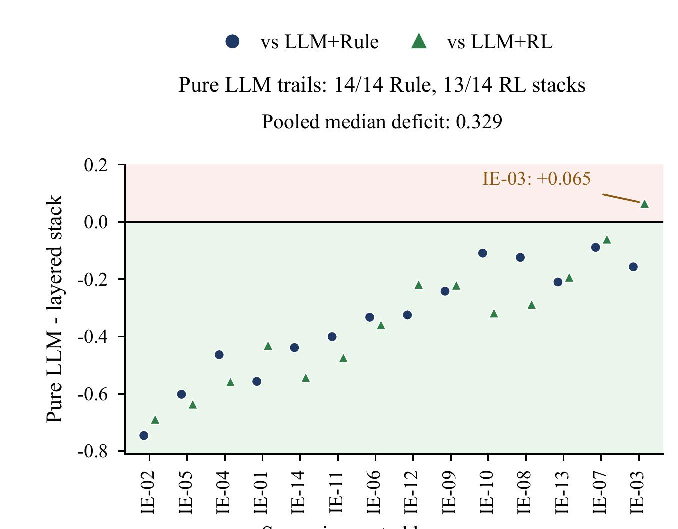
\includegraphics[width=\columnwidth]{figures/fig_hifi_gap_cropped.pdf}
\Description{Scatter of per-scenario composite-score gaps of the pure-LLM stack against each layered stack on the high-fidelity suite; negative gaps indicate the layered stack ahead.}
\caption{End-to-end LLM control deficit: per-scenario composite-score gap of Pure LLM against each layered stack (frozen gap means, ordered by the average of the two gaps; negative = layered stack ahead). Pure LLM trails LLM+Rule on 14/14 and LLM+RL on 13/14 scenarios, with IE-03 the exception; pooled median deficit 0.33.}
\label{fig:hifigap}
\end{figure}

\textbf{Stripping opponent intelligence does not hurt layered stacks.} Removing opponent intelligence (vs.\ the legacy all-knowing prompt) leaves layered stacks essentially unchanged ($+0.000$ LLM+RL, $+0.021$ LLM+Rule) while end-to-end LLM drops $-0.085$; a prompt audit isolates misleading directives in the briefing channel (supplementary Appendix, Headroom Calibration section). Deliberation-layer value is governed by information \emph{quality}, not \emph{quantity}.

\subsection{Mechanism Probe: Layered Value Does Not Require an LLM Information Advantage}\label{sec:mechanism}

We test the competing hypothesis that layered value requires an LLM information advantage with an offline feint-vs-real discrimination probe on the two decoy scenarios (IE-06/IE-11, 400 events each). The result is counterintuitive: the numerical discriminator reaches 84.25\%/90.50\% balanced accuracy vs.\ 51.25\%/45.00\% for the offline LLM ($\Cinfo=-0.330/-0.455$, CIs exclude 0)---the LLM is worse at sensing, yet layered stacks still win on the same scenarios (LLM+Rule $+0.110/+0.066$ and LLM+RL $+0.136/+0.138$ vs.\ the strongest pure baseline). The evidence is thus more consistent with semantic goal decomposition than with an LLM information advantage---why $\Cinfo$ is a diagnostic, not a gate. The probe is offline and scenario-local.

\section{Discussion}\label{sec:discussion}

\subsection{Insights}\label{sec:insights}

\paragraph{I1 --- Layering is conditional, and the conditions are measurable.}
The grid sits at the boundary (decision-form match fails, headroom insufficient); the high-fidelity suite provides evidence for the positive-region hypothesis under the pre-registered design-side admission protocol---falsifiably and by design.

\paragraph{I2 --- Executor floor and decision-form mismatch jointly bound layered value.}
One weak executor floors every planner above it, while the same planners separate under a heuristic executor; on geometrically shaped tasks all three rescue channels fail because the LLM cannot convert semantic understanding into spatial-combinatorial scheduling. Environments crediting LLM deliberation must place difficulty in LLM-strong forms.

\paragraph{I3 --- Layered value comes from semantic goal decomposition, not information advantage.}
The LLM discriminator underperforms a rule baseline ($\Cinfo < 0$), yet layered stacks still win: the evidence is more consistent with the LLM restructuring the task into executable subgoals than with an information advantage.
\paragraph{I4 --- Methodological lessons.}
Pre-registered hypotheses, paired statistics, released traces, and manipulation-validity checks made the boundary confirmation productive: the grid seeded the gates that let the high-fidelity suite (admitted by pre-registered design-side gates) confirm the positive region. Briefing channels should be audited as interface design---the no-intelligence audit isolated misleading directives.

\subsection{Limitations and Threats to Validity}\label{sec:limitations}

\paragraph{Scope of the framework.}
The layering law is domain-agnostic: it applies to any problem whose structure separates a slow, semantic deliberation layer from a fast, continuous execution layer joined by a goal interface; problems without such a time-scale separation are outside its scope by construction. Our instantiations validate both sides (boundary regime and positive region), where the three conditions double as an operational scope test.

\paragraph{Scope and power.}
The grid is minimal-geometry (boundary regime only); high-fidelity covers 14 of 36 interception scenarios, five stacks, one prompt regime. Goal doses are unit-availability, not bits; we do not fit $f$ in Eq.~\ref{eq:law}. Five seeds per LLM stack, three-part stability as the primary gate, Wilcoxon tests corroborating key contrasts ($p<0.002$).

\paragraph{Trust and instrumentation.}
Distributed evaluation cannot verify claimed architectures; rate limits bound but do not eliminate exploitation. Attribution is calibrated on injected and anchored faults; blind \emph{location} of natural faults is a disclosed boundary (\sapp{I}). Replay gates guarantee a recorded trace reproduces under the same configuration, not LLM bit-identical re-emission; the nondeterministic endpoint uses the prompt-level audit and stability criterion (\sapp{D}).

\paragraph{Decision-form and headroom delimitation.}
Decision-form match is a design-side gate anchored by the grid/high-fidelity contrast and the mechanism probe; a 7-scenario check of the $\mathrm{DF}$ prior ($\rho=-0.009$) is too low-powered to claim predictive validity (mid-range validation: \sapp{A}). Headroom is similarly delimited: E1 (120 paired episodes) supports LLM+Rule gains at two of four frozen quantities, but separated tiers were not achieved (95\% CIs straddle zero): calibration feasibility and partial direction confirmation, not a causal test, supported by the boundary regime (P2) and the gain--baseline trend (\sapp{A}).

\section{Conclusion}\label{sec:conclusion}

We formalize decision-stack bifurcation (HSemi-MDP), derive measurable coupling, and distill the conditional layering law: decision-form match, interface carrying, baseline headroom. Validation is two-sided: the grid confirms the boundary prediction (no pay when decision-form match fails and headroom is insufficient), the gate-admitted suite (admitted by pre-registered design-side gates DF/D2/D3, not post-hoc endpoint re-certification) provides evidence for the positive-region hypothesis, and a mechanism probe locates layered value in semantic goal decomposition, not an LLM information advantage. In the evaluated cross-domain setting, the evidence supports placing the LLM at the planning layer above a mature executor rather than using end-to-end LLM control, when the three preconditions jointly provide room for layered gains; environments, traces, and code are released.

\balance
\bibliographystyle{ACM-Reference-Format}
\bibliography{refs}

\end{document}
